\documentclass[varwidth=true, border=2pt]{standalone}
\usepackage{tikz}
\usetikzlibrary{patterns}

\begin{document}
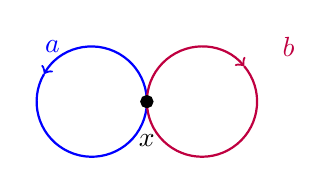
\begin{tikzpicture}[thick]
    \tikzstyle{point}=[circle,thick,draw=black,fill=black,inner sep=0pt,minimum width=4pt,minimum height=4pt]
    \node[blue]   at (4.5, 1.7) {$a$};
    \node[purple] at (7.5, 1.7) {$b$};
    \begin{scope}[xshift=5cm, yshift=1cm]
        \draw[blue,->]   (  0,0)+(150:0.7cm) arc (150:510:0.7cm);
        \draw[purple,<-] (1.4,0)+( 40:0.7cm) arc (40:400:0.7cm);
        \node (z)[point,label={[label distance=0.2cm]-90:$x$}] at (0.7,0) {};
    \end{scope}
\end{tikzpicture}
\end{document}
